% !TeX encoding = UTF-8
% !TeX program = xelatex
% !TeX spellcheck = en_US
%%%%%%%%%%%%%%%%%%%%%%%%%%%%%%%%%%%%%%%%%%%%%%%%%%%%%%%%%%%%%%%%%%%%%%%%%%%%%%%%
%  BeamerJS class demo
%  Institution : Department of Mathematics and Statistics, Université Laval
%  Author : Jerome Soucy
%  email : jerome.soucy@mat.ulaval.ca
%  Unlike BeamerJS.cls, this file may be copied and modified freely, without
%  any condition: it is meant as the starting point of your presentations.
%
%  A short mathematics talk that uses every feature of the class. Each frame
%  states in a comment what it illustrates.
%
%  Compile with: xelatex, biber, xelatex, xelatex (or simply latexmk).
%%%%%%%%%%%%%%%%%%%%%%%%%%%%%%%%%%%%%%%%%%%%%%%%%%%%%%%%%%%%%%%%%%%%%%%%%%%%%%%%
% Options: palette (night, earth, slate, laval), font (charter, baskerville,
% newcm, source, libertinus), footer, noprogress, nosectionpage.
\documentclass[night,charter,footer]{BeamerJS}

% A few macros specific to this document
\newcommand{\N}{\mathbb{N}}
\newcommand{\R}{\mathbb{R}}
\newcommand{\abs}[1]{\left\lvert #1\right\rvert}

% An extra box, created with the class command
\NewBoxJS{conj}{Conjecture}{Accent}{AccentBG}

% Title page
\title[Infinite sums and random points]{Infinite sums and random points}
\subtitle{A guided tour of the BeamerJS class}
\author{First Last}
\position{Position\\Department of Mathematics}
\institute{University}
\event{Department seminar}
\date{October 6, 2026}
\titlelogo{images/logo-example.pdf}

\begin{document}

% Title page: plain and noframenumbering so that it does not count
\begin{frame}[plain,noframenumbering]
	\titlepage
\end{frame}

% Table of contents
\begin{frame}{Outline}
	\tableofcontents
\end{frame}

%%%%%%%%%%%%%%%%%%%%%%%%%%%%%%%%%%%%%%%%%%%%%%%%%%%%%%%%%%%%%%%%%%%%%%%%%%%%%%%%
\section{The harmonic series}
%%%%%%%%%%%%%%%%%%%%%%%%%%%%%%%%%%%%%%%%%%%%%%%%%%%%%%%%%%%%%%%%%%%%%%%%%%%%%%%%
% Each \section automatically produces a section frame.

% defn and notation boxes, \term
\begin{frame}{Partial sums}{The basic vocabulary}
	\begin{defn}[Series]
		Let $(a_n)_{n\geq1}$ be a real sequence. The \term{series} $\sum a_n$
		\term{converges} if the sequence of \term{partial sums}
		\[
			S_N=\sum_{n=1}^{N}a_n
		\]
		has a finite limit as $N\to\infty$.
	\end{defn}

	\begin{notation}
		We write $H_N=\sum_{n=1}^{N}\frac{1}{n}$ for the $N$th harmonic number.
	\end{notation}
\end{frame}

% Theorem, proof, \pause, \stress
\begin{frame}{A divergent series}
	\begin{thm}[Oresme, around 1350]
		The harmonic series $\sum\frac1n$ diverges.
	\end{thm}
	\pause
	\begin{proofbox}
		Group the terms in blocks of length $2^{k}$:
		\[
			H_{2^{m}} = 1+\frac12
			+\underbrace{\frac13+\frac14}_{\geq 1/2}
			+\underbrace{\frac15+\cdots+\frac18}_{\geq 1/2}
			+\cdots
			\;\geq\; 1+\frac{m}{2}.
		\]
		The partial sums are therefore \stress{unbounded}.
		\hfill$\square$
	\end{proofbox}
\end{frame}

% pgfplots: the class colour cycle applies with no extra settings
\begin{frame}{Logarithmic growth}
	\begin{columns}[c,onlytextwidth]
		\begin{column}{0.52\linewidth}
			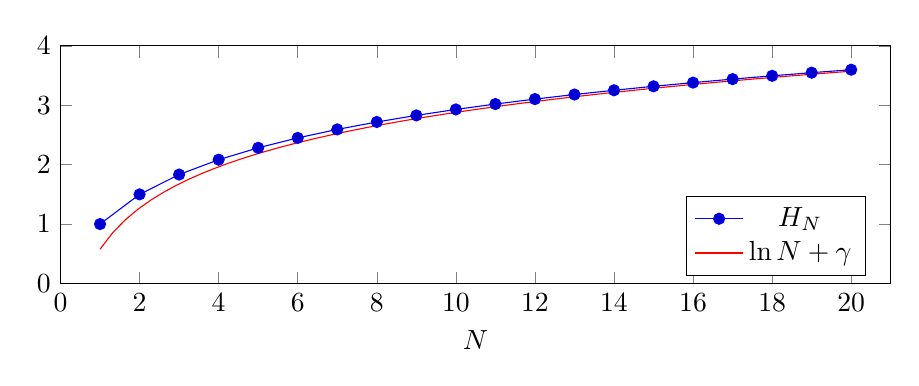
\begin{tikzpicture}
				\begin{axis}[width=\linewidth, height=4.6cm,
						xmin=0, xmax=21, ymin=0, ymax=4,
						xlabel={$N$}, legend pos=south east]
					\addplot coordinates {(1,1.0000) (2,1.5000) (3,1.8333)
						(4,2.0833) (5,2.2833) (6,2.4500) (7,2.5929) (8,2.7179)
						(9,2.8290) (10,2.9290) (11,3.0199) (12,3.1032)
						(13,3.1801) (14,3.2516) (15,3.3182) (16,3.3807)
						(17,3.4396) (18,3.4951) (19,3.5477) (20,3.5977)};
					\addlegendentry{$H_N$}
					\addplot+[no marks, domain=1:20, samples=60]
						{ln(x)+0.5772};
					\addlegendentry{$\ln N+\gamma$}
				\end{axis}
			\end{tikzpicture}
		\end{column}
		\begin{column}{0.44\linewidth}
			\begin{prop}
				\[
					H_N=\ln N+\gamma+o(1),
				\]
				\raggedright
				where $\gamma\approx\num{0.5772}$ is the Euler--Mascheroni
				constant.
			\end{prop}
		\end{column}
	\end{columns}

	\begin{keypoint}
		It diverges, but \highlight{very slowly}: $H_N>10$ takes more than
		\num{12000} terms.
	\end{keypoint}
\end{frame}

%%%%%%%%%%%%%%%%%%%%%%%%%%%%%%%%%%%%%%%%%%%%%%%%%%%%%%%%%%%%%%%%%%%%%%%%%%%%%%%%
\section{The Basel problem}
%%%%%%%%%%%%%%%%%%%%%%%%%%%%%%%%%%%%%%%%%%%%%%%%%%%%%%%%%%%%%%%%%%%%%%%%%%%%%%%%

% Partial outline: the current section is highlighted
\partialtoc

\subsection{Convergence}

% Lemma, corollary, overlays with \only and \uncover
\begin{frame}{The squares converge}
	\begin{lemma}
		For every $n\geq2$, $\dfrac{1}{n^2}<\dfrac{1}{n(n-1)}
		=\dfrac{1}{n-1}-\dfrac{1}{n}$.
	\end{lemma}

	\uncover<2->{%
	\begin{coro}
		$\displaystyle\sum_{n=1}^{\infty}\frac{1}{n^2}
		<1+\sum_{n=2}^{\infty}\Bigl(\frac{1}{n-1}-\frac{1}{n}\Bigr)=2.$
	\end{coro}}

	\only<3>{%
	\begin{rem}
		The telescoping sum only gives a \emph{bound}. The exact value is
		another story.
	\end{rem}}
\end{frame}

% conj box created in the preamble, \bigquote
\begin{frame}{An open question in 1650}
	\begin{conj}[Mengoli, 1650]
		The sum $\sum_{n\geq1}1/n^2$ has a closed form.
	\end{conj}

	Jacob Bernoulli, in Basel, could not crack it. The problem has carried
	the name of his city ever since.

	\bigquote{Read Euler, read Euler, he is the master of us all.}
		{attributed to Pierre-Simon Laplace}
\end{frame}

\subsection{Euler's answer}

% Theorem with a citation, standard beamer blocks
\begin{frame}{The exact value}
	\begin{thm}[Euler, 1734 \cite{euler1740}]
		\[
			\sum_{n=1}^{\infty}\frac{1}{n^2}=\frac{\pi^2}{6}.
		\]
	\end{thm}

	\begin{columns}[T,onlytextwidth]
		\begin{column}{0.48\linewidth}
			\begin{block}{Beamer block}
				Standard blocks follow the palette.
			\end{block}
		\end{column}
		\begin{column}{0.48\linewidth}
			\begin{alertblock}{Alert block}
				Euler's first argument was not fully rigorous.
			\end{alertblock}
		\end{column}
	\end{columns}

	\begin{exampleblock}{Example block}
		Modern proofs can be found in \cite{aigner2018}.
	\end{exampleblock}
\end{frame}

% booktabs table, siunitx, \alert with overlays
\begin{frame}{A numerical check}
	\begin{center}
		\begin{tabular}{r S[table-format=1.6] S[table-format=1.6]}
			\toprule
			{$N$} & {$S_N=\sum_{n\leq N}1/n^2$} & {$\pi^2/6-S_N$} \\
			\midrule
			\num{1}    & 1.000000 & 0.644934 \\
			\num{10}   & 1.549768 & 0.095166 \\
			\num{100}  & 1.634984 & 0.009950 \\
			\num{1000} & 1.643935 & 0.001000 \\
			\bottomrule
		\end{tabular}
	\end{center}

	\begin{itemize}[<+->]
		\item The error is about \alert<2>{$1/N$}.
		\item Each correct digit costs \alert<3>{ten times more} terms.
		\item Euler accelerated the convergence and found
			  $\pi^2/6\approx\num{1.644934}$ by hand.
	\end{itemize}
\end{frame}

% idea box, example, nested lists
\begin{frame}{Euler's idea}
	\begin{idea}
		Treat $\dfrac{\sin x}{x}$ as a polynomial whose roots
		$\pm\pi,\pm2\pi,\dots$ are known.
	\end{idea}

	\begin{enumerate}
		\item Factor:
			$\dfrac{\sin x}{x}=\prod_{k\geq1}\Bigl(1-\dfrac{x^2}{k^2\pi^2}\Bigr)$.
		\item Compare the coefficients of $x^2$:
			\begin{itemize}
				\item on the left, the Taylor series gives $-\frac16$;
				\item on the right, the product gives $-\sum_k\frac{1}{k^2\pi^2}$.
			\end{itemize}
	\end{enumerate}

	\begin{ex}
		The same argument gives $\sum 1/n^4=\pi^4/90$.
	\end{ex}
\end{frame}

%%%%%%%%%%%%%%%%%%%%%%%%%%%%%%%%%%%%%%%%%%%%%%%%%%%%%%%%%%%%%%%%%%%%%%%%%%%%%%%%
\section{Random points}
%%%%%%%%%%%%%%%%%%%%%%%%%%%%%%%%%%%%%%%%%%%%%%%%%%%%%%%%%%%%%%%%%%%%%%%%%%%%%%%%

% \JSscatter, \JSpoissonScatter, \JSlastN, custom point style
\begin{frame}{Two ways to scatter points}
	\begin{columns}[T,onlytextwidth]
		\begin{column}{0.48\linewidth}
			\centering
			\begin{tikzpicture}
				\JSscatter{5}{3.4}{40}{7}
			\end{tikzpicture}\\[0.3em]
			{\small\sffamily\color{Secondary}exactly 40 points}
		\end{column}
		\begin{column}{0.48\linewidth}
			\centering
			\begin{tikzpicture}
				\JSpoissonScatter[pointJS, fill=Primary]{5}{3.4}{2.35}{11}
			\end{tikzpicture}\\[0.3em]
			{\small\sffamily\color{Secondary}%
			 $N\sim\mathrm{Poisson}(40)$; here $N=\JSlastN$}
		\end{column}
	\end{columns}

	\begin{defn}[Homogeneous Poisson process]
		For every region $A$, the number of points in $A$ follows a Poisson
		law with parameter $\lambda\abs{A}$, and disjoint regions receive
		independent counts \cite{kingman1993}.
	\end{defn}
\end{frame}

% framedbox (free title), fontawesome
\begin{frame}{Why Poisson?}
	\begin{columns}[T,onlytextwidth]
		\begin{column}{0.47\linewidth}
			\begin{framedbox}{\faIcon{th} Fine grid}
				Cut the window into $m$ small cells; each one receives a point
				with probability $\lambda\abs{A}/m$.
			\end{framedbox}
		\end{column}
		\begin{column}{0.47\linewidth}
			\begin{framedbox}{\faIcon{infinity} Taking the limit}
				The total count is binomial, and tends to
				$\mathrm{Poisson}(\lambda\abs{A})$ as $m\to\infty$.
			\end{framedbox}
		\end{column}
	\end{columns}

	\begin{keypoint}
		The starting point: \stress{independent cells}. Everything else
		follows.
	\end{keypoint}
\end{frame}

%%%%%%%%%%%%%%%%%%%%%%%%%%%%%%%%%%%%%%%%%%%%%%%%%%%%%%%%%%%%%%%%%%%%%%%%%%%%%%%%
\section{Toolbox}
%%%%%%%%%%%%%%%%%%%%%%%%%%%%%%%%%%%%%%%%%%%%%%%%%%%%%%%%%%%%%%%%%%%%%%%%%%%%%%%%

% \palettepreview: the four palettes side by side
\begin{frame}{Four palettes}{Chosen with a class option}
	\begin{columns}[c,onlytextwidth]
		\begin{column}{0.45\linewidth}
			\palettepreview{night}\par\medskip
			\palettepreview{earth}\par\medskip
			\palettepreview{slate}\par\medskip
			\palettepreview{laval}
		\end{column}
		\begin{column}{0.52\linewidth}
			\begin{itemize}
				\item Primary, secondary, accent, background.
				\item Everything follows: titles, boxes, plots, links.
			\end{itemize}
			{\footnotesize\ttfamily\textbackslash documentclass[earth]\{BeamerJS\}}
			\vskip0.6em
			\JSrule
		\end{column}
	\end{columns}
\end{frame}

% allowframebreaks: the content spreads over several frames and the title
% gets "(continued)". \framebreak forces a break at a specific place.
\begin{frame}[allowframebreaks]{Cheat sheet}
	\small
	\term{Environments}\par
		\begin{tabular}{@{}>{\ttfamily\small}l l@{}}
			defn & definition \\
			thm, prop, lemma, coro & results (optional name in brackets) \\
			proofbox & proof \\
			ex, rem & example, remark \\
			idea, notation & icon boxes \\
			framedbox\{Title\} & framed box with a free title \\
			keypoint & the take-away sentence \\
		\end{tabular}
	\medskip

	\term{Title page}\par
		\begin{tabular}{@{}>{\ttfamily\small}l l@{}}
			\textbackslash position\{...\} & job title \\
			\textbackslash event\{...\} & conference, seminar \\
			\textbackslash titlelogo\{file\} & logo on the left \\
		\end{tabular}
	\medskip

	\framebreak

	\term{Commands}\par
		\begin{tabular}{@{}>{\ttfamily\small}l l@{}}
			\textbackslash term, \textbackslash highlight, \textbackslash stress
				& emphasis \\
			\textbackslash bigquote\{quote\}\{author\} & displayed quotation \\
			\textbackslash partialtoc[title] & partial outline \\
			\textbackslash NewBoxJS & create a box \\
			\textbackslash JSscatter, \textbackslash JSpoissonScatter & point clouds \\
			\textbackslash palettepreview\{name\} & palette preview \\
			\textbackslash startappendix, \textbackslash stopappendix & appendix frames \\
		\end{tabular}
	\medskip

	\begin{rem}
		Every name also has a French version (\texttt{lemme}, \texttt{lumiere},
		\texttt{\textbackslash defi}, \texttt{\textbackslash planpartiel}…):
		see section 16 of \texttt{BeamerJS.cls}.
	\end{rem}
\end{frame}

% Bibliography
\begin{frame}{References}
	\printbibliography
\end{frame}

% Appendix: numbering frozen, progress bar hidden
\startappendix

\begin{frame}{Appendix: the tail of the series}
	\begin{prop}
		For every $N\geq1$,
		\[
			\frac{1}{N+1}<\sum_{n>N}\frac{1}{n^2}<\frac{1}{N}.
		\]
	\end{prop}
	\begin{proofbox}
		Use
		\[
			\frac{1}{n(n+1)}<\frac{1}{n^2}<\frac{1}{n(n-1)}
		\]
		and sum the two telescoping series. \hfill$\square$
	\end{proofbox}
\end{frame}

\stopappendix

\end{document}
